\chapter{Magazyn i jego rola w procesach logistycznych}
\label{c4:c4}

	Gospodarka magazynowa zajmuje się głównie procesami decyzyjnymi, w wyniku których następuje 
	zmiana struktury zapasów w magazynie. Magazyn utożsamiany jest jako bufor znajdujący się
	między strefą przyjęć, a strefą wydań, którego głównym celem jest niwelowanie
	różnic wynikających z przewagi podaży nad popytem lub sytuacji odwrotnej. Sytuacja idealna
	oczywiście zakłada brak konieczności posiadania magazynu i ciągłego, jednolitego przepływu
	produktów od strefy przyjęć do strefy wydań. Niestety jest ona jest niemożliwa i bardzo
	rzadko można obserwować aby podaż i popyt były jednakowe. Tak więc magazyn - bufor jest
	wynikiem różnic w strukturze przepływu dóbr na wejściu i wyjściu. 
	Jeśli zdefiniować magazyn jako element niepożądany w łańcuchu dostaw, można dojść do wniosku, 
	że zapasy same w sobie są niepożądane.

	\paragraph{Funkcje zapasów, czyli zadania magazynowania}:
	\begin{itemize}
		\item niwelowanie różnic między popytem a podążą;
		\item wykorzystanie efektu skali, czyli zamówienie oraz odbiór większej ilości towaru celem uzyskania
		rabatów;
		\item zabezpieczenie przed niepewnością, nieprzewidywanymi zmianami na rynku;
		\item spekulacje, gromadzi się większe ilości towaru niż to potrzebne, które następnie sprzedaje się
		w okresie tzw. dołka za ceny wyższe, ale wciąż mniejsze niż konkurenci \cite{systemyLogistyczne_pfohl}.
	\end{itemize}		
	 
\section{Rola magazynu w łańcuchu dostaw}
	\begin{quotation}
		\textit{
			``Magazyn jest jednostką funkcjonalno-organizacyjną, przeznaczoną do magazyno\-wania
			dóbr materialnych (zapasów) w wyodrębnionej przestrzeni, budowli magazynowej, według ustalonej
			technologii, wyposażoną w odpowiednie urządzenia i środki techniczne, zarządzaną i obsługiwaną
			przez zespół ludzi, wyposażonych w odpowiednia umiejętności \footnote{PN-N-01800:1984 \cite{norm_warehouse_defintion}}.''
		}
	\end{quotation}
	
	Wobec tego magazyn nie jest jedynie statycznym bytem łańcuchów logistycznych, ale jego integralną
	częścią bez której żadne przedsiębiorstwo, w szczególności produkcyjne, nie mogłoby sprawnie
	funkcjonować. Ogół czynności, czyli \textbf{magazynowanie}. jest tym, co związane jest z manipulowaniem
	zapasami oraz ich przechowywanie. Czynności te mogą odnosić się zarówno do początkowej fazy procesów gospodarczych
	u producenta danego dobra, znajdować się pośrodku łańcucha logistycznego jako magazyn centralny, bądź u klienta
	końcowego, hurtownika. Niezależnie od miejsca występowania magazynowanie zdefiniowane jest przez cztery
	podstawowe punkty: 
	\begin{itemize}
		\item przyjęcie,
		\item składowania,
		\item kompletacja,
		\item wydanie \cite{PZMW}\cite{PL_FM}.
	\end{itemize}
	
	\subsection{Magazynowania jako proces magazynowanie}
		\paragraph{Przyjęcie} jest wydarzeniem zewnętrznym, które rozpoczyna cały ciąg czynności 
		związany\-ch z przetwarzaniem go. Warto w tym miejscu zaznaczyć, że faza przyjęcia nie jest 
		równoważna z wprowadzaniem danych o przyjmowanych dobrach do magazynu i uaktualnieniu stanów. 
		Zanim to nastąpi należy rozładować produkty oraz poddać je kontroli zarówno jakościowej i ilościowej.
			\subparagraph{Kontrola ilościowa} czyli sprawdzeniu stanu faktycznego z oczekiwanym, 
			zgodnie ze \-stanem np. dokumentu przewozowego. 
			Sprawdzenie to przyjmuje różne formy, które są najczęściej uzależnione od rodzaju artykułu. 
			Różnicę łatwo wskazać
			poprzez porównanie produktów takich jak zboża (\textit{produkt sypki}) czy bele papieru. 
			W pierwszym przypadku 
			kontrola ilościowa prawdopodobnie przebiegnie z użyciem wagi samochodowej, a w drugim przypadku 
			zostanie zliczona
			ilość sztuk beli.  
			\subparagraph{Kontrola jakościowa} wykazuje z drugiej strony bezpośrednie i silne powiązanie z wymaganiami prawnymi bądź
			różnorodnymi normami odnoszącymi się do danego rodzaju dóbr. Dla większości produktów jest to kontrola
			wzrokowa w poszukiwaniu uszkodzeń mechanicznych, wycieków itp. Niemniej warto nadmienić, że w przypadku
			artykułów, których natura jest szkodliwa dla ludzi, zwierząt, taka kontrola może potrwać niejednokrotnie
			więcej niż jeden dzień i wymagać przeprowadzenia badań laboratoryjnych.
		\paragraph{Składowanie} polega na usystematyzowanym umieszczaniu dóbr materialnych, które najczęściej przyjmują
		postać jednostek ładunkowych (\textit{palety EURO}), w przestrzeni magazynu. Czynność ta, jako będąca właściwie
		esencją każdego z magazynów, jest bardzo rozbudowana, przez co wspomagana przez różnego rodzaju urządzania, począwszy
		od wózków widłowych, pasów transmisyjnych po regały dowolnego typu. Z tego powodu strefy składowania dzielą się na:
		\begin{enumerate}
			\item \textbf{strefy składowania} - wydzieloną przestrzeń służącą do 
			przechowywanie zapasów w urządzeniach bądź piętrzenia w stosy
			\item \textbf{strefy manipulacyjnej} - wszystkie drogi manipulacyjne 
			oraz przejazdowe nie będące przestrzenią składowania
		\end{enumerate}	
		W tym miejscu należy zwrócić uwagę na konieczność uwzględnienia takich właściwości fizycznych oraz chemicznych, które
		mają bezpośrednie przełożenie na warunki, w jakich należy składować dane dobra. Do takich parametrów należą
		chociażby:
		\begin{enumerate}
			\item temperatura, wilgotność powietrza
			\item właściwości trujące, wybuchowe materiałów itp\footnote{Decydują o tym wymogi prawne \cite{ustawa_flamableMaterials}}
			\item odporność na zgniatanie \footnote{szczególnie ważna w przypadku piętrzenia w stosy}
		\end{enumerate}			
		Wynika z tego także, że składowania jest ważnym elementem magazynowania, ponieważ to od tego, czy zostanie
		wykonane poprawnie, zależy czy towar zostanie uszkodzony bądź nie \cite{EWSS}.
	\paragraph{Kompletacja} \label{c4:kompletacja} jest działaniem, które najczęściej występuje w momencie rozpoczęcia procedury
	wydawania towaru. Polega ona na pobraniu z posiadanych zapasów takich materiałów i w takiej ilości, jakie
	wynikają z realizowanego zamówienia. Warto w tym miejscu nadmienić, że zamówienie może mieć zarówno
	charakter \textbf{zewnętrzny} lub \textbf{wewnętrzny}. Niedopuszczalne są w tym momencie jakiekolwiek odstępstwa. Innymi słowy
	magazynier, jeśli kompletacja realizowana jest przez człowieka, nie ma prawa pobrać większej ilości elementów niż
	jest to potrzebne. Z drugiej strony sytuacja, kiedy elementów byłoby za mało w magazynie, również nie 
	powinna mieć miejsca. Z pobranych jednostek formuje się jednostki ładunkowe, którymi mogą być np
	\begin{itemize}
		\item kartony,
		\item palety ładunkowe.
	\end{itemize}
	Uznaje się, że to jest zdecydowanie najtrudniejsza faza, gdzie jej trudność wynika z błędu człowieka, który zajmuje się
	procesem kompletacji. Dlatego coraz częściej spotyka się systemy automatycznej kompletacji współpracujące z magazynami
	wysokiego składu (które również często pracują w trybie automatycznym), aby to one dokonały kompletacji. W tym rozwiązaniu
	magazynier potrzebny jest jedynie, aby zeskanować lub wprowadzić informacje o aktualnie ładowanej jednostce ładunkowej, aby
	poinformować system, że zdjął ją ze strefy postojowej i umieścił w wyznaczonym miejscu (np. na podstawionym samochodzie
	dostawczym). 	
	\paragraph{Wydawanie} dóbr materialnych jest finalną fazę całego procesu magazynowania. 
	Jak zosta\-ło wspomniane, kompletacja polega na zgromadzeniu określonej ilości dóbr. W tym miejscu
	ważne jest to, czy wspomniane dobra zostały zmodyfikowane. Modyfikacja w tym sensie odnosi się do ustalenia, czy produkty
	powstały w wyniku kompletacji, produkcji, czy też są wydawane identycznej postaci, w jakiej zostały przyjęte. Zależnie
	od tego, dobra mogą zostać wydane lub należy je odpowiednio zabezpieczyć. Jednym z popularniejszych rozwiązań jest użycie
	pasów zabezpieczających bądź folii stretch. Oba te rozwiązania znaczącą podnoszą zwartość oraz stabilność ładunku, co
	przekłada się na mniejsze prawdopodobieństwo uszkodzenia towaru. Odbiorcy, i nie jest to wcale zdarzenie jednostkowe,
	mogą często wybrać formę transportu produktu, czyli innymi słowy dobra muszą zostać odpowiednio zabezpieczone i zapakowane,
	aby można je było wysłać to klienta. 
		\subparagraph{Kontrola} jest tutaj koniecznością. Osoba wyznaczona ma obowiązek zweryfikować 
		popra\-wność załadunku pod kątem bezpieczeństwa zarówno ładunku, jak i sposobu jego 
		zabezpieczenia. Dopiero pozytywna weryfikacja oznacza możliwość umieszczenia
		towarów na podstawionym samochodzie transportowym \cite{PL_FM}.
		
	\subsection{Podział magazynu na strefy - cele i korzyści}
		\begin{figure}[h]
			\centering
			
\includegraphics[width=0.95\textwidth]{images/warehouse_simple_schema}
			\caption[Obszary magazynu - układ uproszczony]{
				Uproszczony układ magazynu z podstawowymi strefami\\
				źródło: opracowanie własne na podstawie \cite{systemyLogistyczne_pfohl}
			}
			\label{c4:warehouse_simple_schema}
		\end{figure}
		Zgodnie z rysunkiem powyżej, w magazynie występują zawsze strefy, z których każda odpowiada danej
		części procesu magazynowania. I tak mamy więc strefę \textbf{przyjęć}, \textbf{składowania}, \textbf{kompletacji} oraz \textbf{wydań}.
		
		\paragraph{Strefa przyjęć} jest pierwszą ze stref, w których będzie znajdował się produkt podczas pobytu w magazynie. 
		Właśnie w tej strefie wykonuje się następujące zadania: rozładunek dostarczonych towarów, identyfikacje, kontrolę jakościową
		oraz ilościową, czy też przystosowanie do magazynowania. Operacjami mający największy priorytet są skontrolowanie
		towaru oraz przystosowanie do magazynowania. Ważnym elementem, który w pewien sposób wyznacza efektywność tej strefy, jest
		czas. Towary powinny znajdować się w fazie przyjęcia możliwie najkrócej.
		\paragraph{Strefę składowania towaru} można uznać za całkowite przeciwieństwo strefy przyjęć. Nie ma presji czasu, 
		natomiast ważne stają się procesy składowania towaru, która opuszczają, najczęściej, towary w tej samej formie,
		w jakiej zostały do magazyny wprowadzone. Magazyny mają duży potencjał do wprowadzenia obsługi automatycznej. 
		Ponieważ prócz operacji składowania muszą one zapewnić jednocześnie możliwość wydań / przyjęć tym bardziej odpowiednie,
		wydaje się zautomatyzowanie i tych operacji. 
		\paragraph{Strefa kompletacji} jest przedostatnim miejscem przed opuszczeniem magazynu. Ta strefa charakteryzuje się
		podobnymi właściwościami co strefa przyjęć. Niedopuszczone jest prze\-trzymywanie produktów w tej strefie dłużej niż jest 
		to wymagane. Z uwagi na dzisiejszą dynamiką działań w łańcuchach dostaw, takie podejście mogłoby skutkować zablokowaniem
		magazynu. Jest to sprzeczne z występującym jeszcze w wielu firmach podejściem ręcznej kompletacji w tej strefie. Ogólnie
		towar, który wchodzi to strefy kompletacji powinien ją opuścić w innej formie niż się w niej znalazł. Mając na myśli formę,
		należy mieć na uwadze przystosowanie towarów do transportu w dany sposób. Przykładowo jeśli towar przechowywane jest w magazynie
		w jednostkach zbiorczych typu karton tekturowy, może się okazać przydatne umieszczenie takich kartonów na paletowej 
		jednostce ładunkowej o standardowych wymiarach. 
		\paragraph{Strefa wydań} to ostatnie miejsce na drodze towaru. Produkty tutaj trafiające bardzo często znajdują się już
		na paletowych jednostkach ładunkowych bądź innego rodzaju zbiorczych jednostkach ładunkowych. Magazynowy
		obszar wyjścia obejmuje swym zasięgiem procesy, których zadaniem jest przygotowanie i wysyłka dóbr do odbiorcy. 
		Do tych zadań należą między innymi:
		\begin{itemize}
			\item odebranie towarów z pakowni,
			\item uporządkowanie według zadanego kryterium,
			\item kierowanie operacją załadunku.
		\end{itemize}
		\begin{figure}[h]
			\centering
			\begin{subfigure}[b]{0.3\textwidth}
                \centering
                
\includegraphics[width=\textwidth]{images/przeplywowy_magazyn}
                \caption{Przepływowy}
                \label{fig:linear_warehouse}
        	\end{subfigure}
        	\quad
			\begin{subfigure}[b]{0.3\textwidth}
                \centering
                
\includegraphics[width=\textwidth]{images/workowy_magazyn}
                \caption{Workowy}
                \label{fig:baggy_warehouse}
        	\end{subfigure}
        	\quad
			\begin{subfigure}[b]{0.3\textwidth}
                \centering
                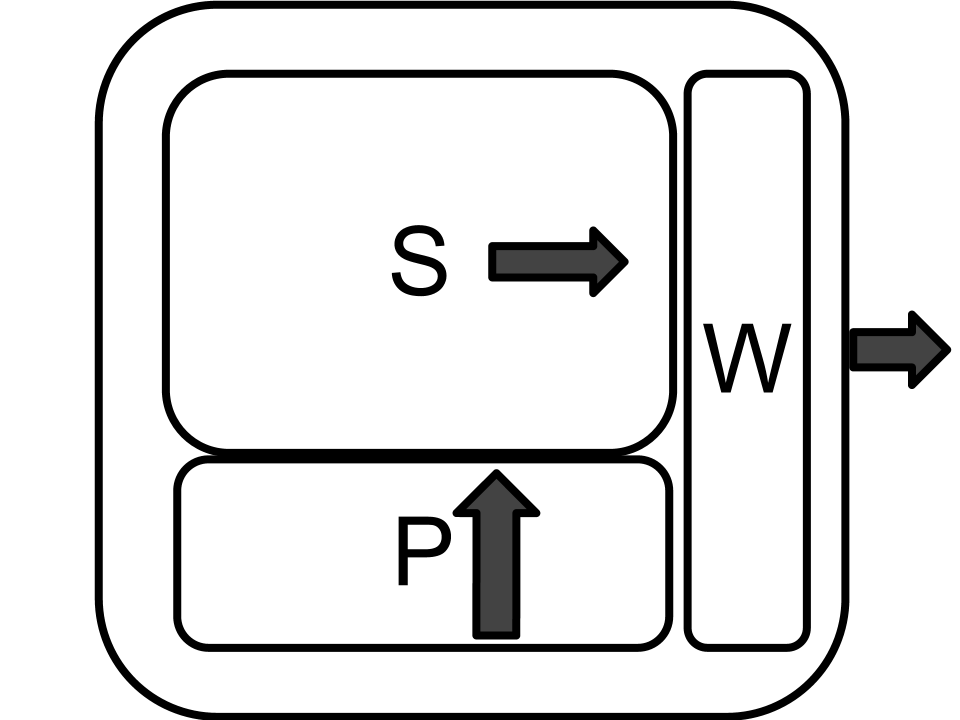
\includegraphics[width=\textwidth]{images/katowy_magazyn}
                \caption{Kątowy}
                \label{fig:angle_warehouse}
        	\end{subfigure}
        	\caption[Układy technologiczne magazynów]{
				Układy technologiczne magazynów\\
				źródło: \cite{PL_FM}        	
        	}
		\end{figure}
		\paragraph{Układy technologiczne} są innym podejściem dla strukturalnego opisania magazynu i odnoszą się
		one do fizycznego przepływu produktów w magazynie. W układzie liniowym \footnote{Rysunek \ref{fig:linear_warehouse}} 
		charakterystyczne jest to, że zarówno strefy wydań, jak i przyjęć znajdują się po przeciwnych stronach. Dla kontrastu,
		w układzie workowym \footnote{Rysunek \ref{fig:baggy_warehouse}} te strefy znajdują się obok siebie i niejednokrotnie
		stanowią jedność. Nie jest to błąd, a nawet można uznać to za całkiem przydatne rozwiązanie. Korzyścią, jaka 
		wynika z takiego rozmieszczenia jest możliwość używania tych samych urządzeń transportowo-przeładunkowych zarówno
		podczas przyjęć, jak i wydań. 
	
\section{Zarządzanie magazynem}
	Zarządzanie magazynem sprowadza się do spełnienia wszystkich jego parametrów użyt\-kowych, jakimi są:
	zapewnienie wymaganego poziomu obsługi klienta, przy jednoczesnym akceptowalnym poziomie kosztów magazynowanie.
	W tym wypadku akceptowalny, nie znaczy najniższy. Ważne jest to, aby nie dopuścić do uszkodzenia magazynowanych
	dóbr i jednocześnie utrzymać pożądanych poziom kosztów.
	Realizacja tego celu jest możliwa jeśli \textbf{zarządzanie magazynem} odbywa się zgodnie z cyklem
	przedstawionym na schemacie \ref{fig:warehouse_management_algorithm}, który z kolei jest odpowiedzią na
	następujące pytania, pochodzące z teorii i inżynierii systemów:
	\begin{itemize}
		\item gdzie jesteśmy ?
		\item dokąd zmierzamy ?
		\item jak zamierzamy się tam dostać ?
		\item skąd wiemy, że dotarliśmy ?
	\end{itemize}
	\begin{figure}[H]
		\centering
		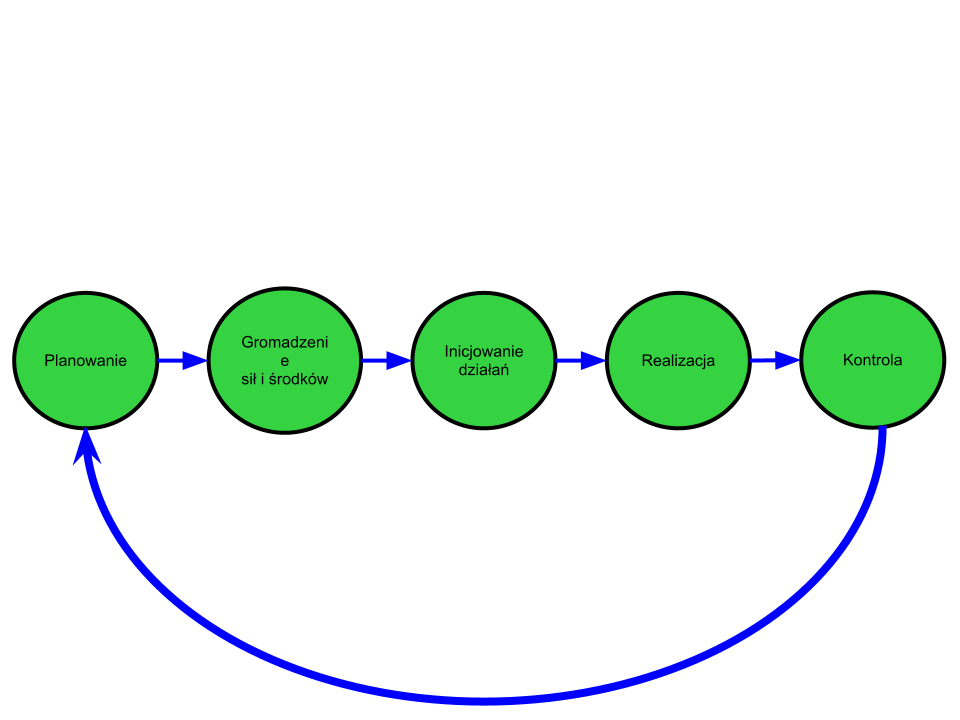
\includegraphics[width=0.95\textwidth]{images/warehouse_management_algorithm_2}
		\caption[Cykl operacji zarządzania magazynem]{
			Cykl operacji zarządzania magazynem w oparciu o teorię systemów \\
			źródło: opracowanie własne na podstawie \cite{PZMW}
		}
		\label{fig:warehouse_management_algorithm}
	\end{figure}
	Samo działanie magazynu opiera się na realizacji czynności czysto fizycznych, związanych z zadaniami transportowymi 
	i towarzyszących im informacji \cite{PZMW}. Organizacja faz procesów magazynowania jest ukierunkowana głównie na
	optymalizację wykorzystania przestrzeni magazynowej, racjonalizację rozmieszczenia procesów magazynowania oraz
	ostatecznie minimalizację strat powstających podczas samej fazy składowania. Racjonalne wykorzystanie
	przestrzeni magazynowej jest możliwe jedynie, gdy spełnione są następujące warunki:
	\begin{enumerate}
		\item jednocześnie wysokie są wskaźniki wykorzystania powierzchni, wysokości strefy składowania;
		\item zapewniony jest jak najprostszy dostęp do wszystkich pozycji asortymentowych. Ten postulat
		realizowany jest poprzez dobranie odpowiednich rodzajów regałów oraz struktury samego magazynu;
		\item swobodne oraz, co ważniejsze, bezpieczne procesy przemieszczenia dóbr stosowanymi
		w procesie magazynowania urządzeniami do transportu w strefie składowania \cite{logistyka_w_przedsiebiorstwie}.
	\end{enumerate}